\documentclass{article}
\usepackage[paperwidth=16in, paperheight=9in, margin=0.4in]{geometry}
\usepackage{tikz}
\usetikzlibrary{positioning, arrows.meta, calc, decorations.pathmorphing}
\usepackage{amsmath,amssymb}
\usepackage{xcolor}
\usepackage{pifont}

\definecolor{hexgreen}{HTML}{388E3C}
\newcommand{\cmark}{\textcolor{hexgreen}{\ding{51}}}
\newcommand{\xmark}{\textcolor{hexred}{\ding{55}}}

\definecolor{hexteal}{HTML}{2C9CA0}
\definecolor{hexrose}{HTML}{D77A7E}
\definecolor{hexred}{HTML}{C81223}
\definecolor{hexblue}{HTML}{2665EA}
\definecolor{hexgray}{HTML}{999999}
\definecolor{hexpink}{HTML}{F0C5C9}
\definecolor{hexblack}{HTML}{000000}

% Color aliases for TikZ box style matching - All borders mapped to hexblack
\colorlet{hextealborder}{hexblack}
\colorlet{hextealbg}{hexteal!10}
\colorlet{hexredborder}{hexblack}
\colorlet{hexredbg}{hexpink!50}
\colorlet{hexblueborder}{hexblack}
\colorlet{hexbluebg}{hexblue!10}
\colorlet{hexroseborder}{hexblack}
\colorlet{hexrosebg}{hexpink!30} % Softened to 30% for improved text contrast
\colorlet{hexgrayborder}{hexblack}
\colorlet{hexgraybg}{hexgray!15}

\pagestyle{empty}

\begin{document}
\centering
\vspace*{\fill}
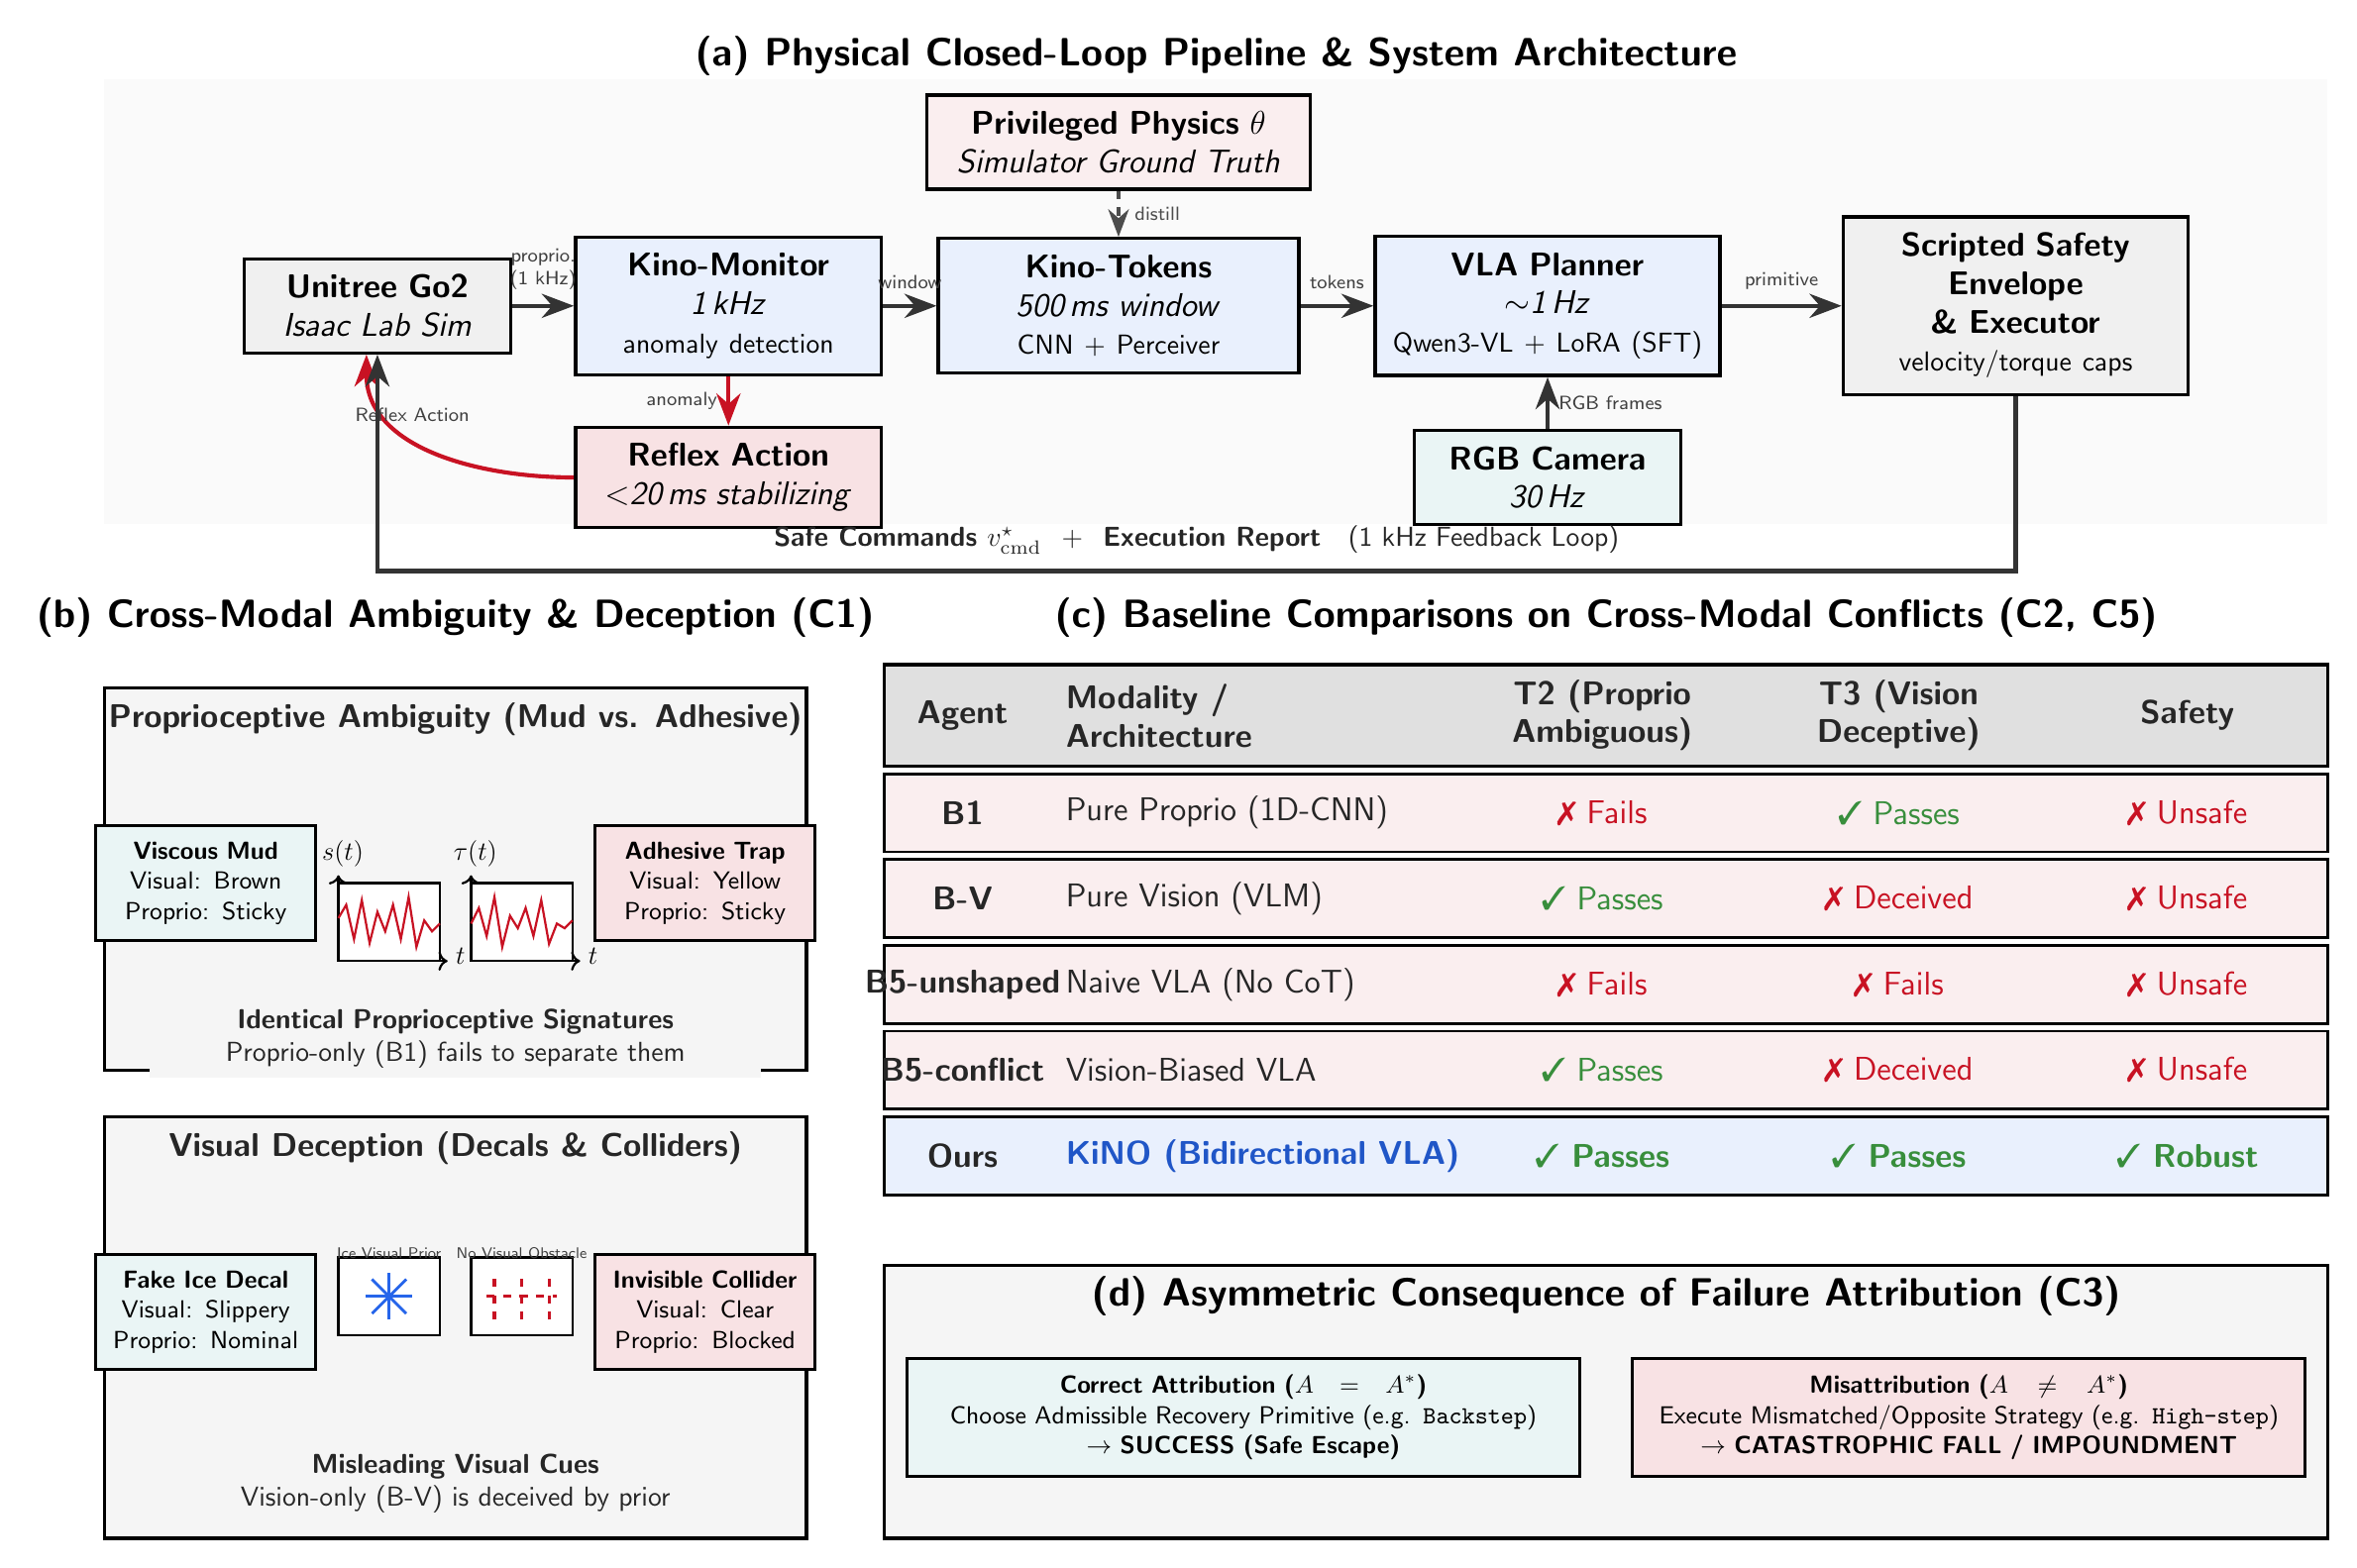
\begin{tikzpicture}[
  font=\sffamily\large,
  box/.style={rectangle, draw=#1border, fill=#1bg, line width=1.2pt, align=center, inner sep=6pt}, % Sharp rectangles
  title/.style={font=\sffamily\bfseries\Large, text=hexblack},
  subtitle/.style={font=\sffamily\bfseries\large, text=hexblack!85},
  lab/.style={font=\sffamily\normalsize, text=hexblack!85, align=center},
  smalllab/.style={font=\sffamily\scriptsize, text=hexblack!75, align=center},
  arrow/.style={-{Stealth[scale=1.2]}, line width=1.5pt, hexblack!80},
  redarrow/.style={-{Stealth[scale=1.2]}, line width=1.5pt, hexred}, % Red arrow
]

% ==================== PART (a): PHYSICAL PIPELINE & SYSTEM ====================
\node[title] (titleSys) at (13.25, 10.8) {(a) Physical Closed-Loop Pipeline \& System Architecture};

% System pipeline border background only (removed outer border black line)
\fill[hexgray!5] (-1.0, 4.8) rectangle (27.5, 10.5);

% Shifted all components right by 2.0 units to balance left/right margins at exactly 2.0 units
\node[box=hexgray, text width=3.0cm, minimum height=1.2cm] (robot) at (2.5, 7.6) {\textbf{Unitree Go2}\\\textit{Isaac Lab Sim}};
\node[box=hexblue, text width=3.5cm, minimum height=1.2cm] (mon) at (7.0, 7.6) {\textbf{Kino-Monitor}\\\textit{1\,kHz}\\\normalsize anomaly detection};
\node[box=hexblue, text width=4.2cm, minimum height=1.2cm] (tok) at (12.0, 7.6) {\textbf{Kino-Tokens}\\\textit{500\,ms window}\\\normalsize CNN + Perceiver};
\node[box=hexblue, text width=4.0cm, minimum height=1.2cm] (vla) at (17.5, 7.6) {\textbf{VLA Planner}\\\textit{$\sim$1\,Hz}\\\normalsize Qwen3-VL + LoRA (SFT)};
\node[box=hexgray, text width=4.0cm, minimum height=1.2cm] (env) at (23.5, 7.6) {\textbf{Scripted Safety}\\\textbf{Envelope \& Executor}\\\normalsize velocity/torque caps};

% Distillation - using hexrose, labeled with 'distill'
\node[box=hexrose, text width=4.5cm, minimum height=0.8cm, draw=hexroseborder, fill=hexrosebg] (theta) at (12.0, 9.7) {\textbf{Privileged Physics $\theta$}\\\textit{Simulator Ground Truth}};
\draw[arrow, dashed, line width=1.2pt, hexblack!70] (theta) -- node[smalllab,right,text=hexblack!70,xshift=2pt]{distill} (tok);

% Vision input - using hexteal
\node[box=hexteal, text width=3.0cm, minimum height=0.8cm, draw=hextealborder, fill=hextealbg] (camera) at (17.5, 5.4) {\textbf{RGB Camera}\\\textit{30\,Hz}};
\draw[arrow] (camera) -- node[smalllab,right]{RGB frames} (vla);

% Reflex loop - using hexred
\node[box=hexred, text width=3.5cm, minimum height=0.8cm, draw=hexredborder, fill=hexredbg] (reflex) at (7.0, 5.4) {\textbf{Reflex Action}\\\textit{$<$20\,ms stabilizing}};
\draw[redarrow] (mon) -- node[smalllab,left]{anomaly} (reflex);
\draw[redarrow] (reflex.west) to[out=180,in=-90] node[smalllab,above,pos=0.6,yshift=2pt]{Reflex Action} ([xshift=-4pt]robot.south);

% Main arrows
\draw[arrow] (robot) -- node[smalllab,above,yshift=2pt]{proprio.\\(1 kHz)} (mon);
\draw[arrow] (mon) -- node[smalllab,above,yshift=2pt]{window} (tok);
\draw[arrow] (tok) -- node[smalllab,above,yshift=2pt]{tokens} (vla);
\draw[arrow] (vla) -- node[smalllab,above,yshift=2pt]{primitive} (env);

% Feedback Loop
\draw[arrow] (env.south) -- (23.5, 4.2)
  -- node[lab,above,yshift=2pt]{\textbf{Safe Commands $v_{\mathrm{cmd}}^{\star}$ \ $+$ \ Execution Report} \ \ (1 kHz Feedback Loop)} (2.5, 4.2)
  -- (robot.south);


% ==================== PART (b): CROSS-MODAL CHALLENGES ====================
\node[title] (titleA) at (3.5, 3.6) {(b) Cross-Modal Ambiguity \& Deception (C1)};

% Proprioceptive Ambiguity Panel - Aligned top to y=2.7 (matches part c table top)
\draw[hexblack, fill=hexgray!10, line width=1.2pt] (-1.0, -2.2) rectangle (8.0, 2.7);
\node[subtitle] at (3.5, 2.3) {Proprioceptive Ambiguity (Mud vs. Adhesive)};

\node[box=hexteal, text width=2.4cm, font=\sffamily\small] (mud) at (0.3, 0.2) {\textbf{Viscous Mud}\\Visual: Brown\\Proprio: Sticky};
\node[box=hexred, text width=2.4cm, font=\sffamily\small] (glue) at (6.7, 0.2) {\textbf{Adhesive Trap}\\Visual: Yellow\\Proprio: Sticky};

% Mud waveform - added realistic experimental noise
\begin{scope}[shift={(2.0, -0.8)}]
  \draw[hexblack, line width=0.8pt, fill=white] (0,0) rectangle (1.3,1.0);
  \draw[->, line width=0.8pt] (0,0) -- (1.4,0) node[right, scale=0.8, yshift=2pt] {$t$};
  \draw[->, line width=0.8pt] (0,0) -- (0,1.1) node[above, scale=0.8, xshift=2pt] {$s(t)$};
  \draw[line width=0.8pt, hexred] (0,0.55) -- (0.1,0.72) -- (0.2,0.28) -- (0.3,0.78) -- (0.4,0.23) -- (0.5,0.63) -- (0.6,0.38) -- (0.7,0.72) -- (0.8,0.28) -- (0.9,0.82) -- (1.0,0.18) -- (1.1,0.52) -- (1.2,0.38) -- (1.3,0.48);
\end{scope}

% Adhesive waveform - added realistic experimental noise
\begin{scope}[shift={(3.7, -0.8)}]
  \draw[hexblack, line width=0.8pt, fill=white] (0,0) rectangle (1.3,1.0);
  \draw[->, line width=0.8pt] (0,0) -- (1.4,0) node[right, scale=0.8, yshift=2pt] {$t$};
  \draw[->, line width=0.8pt] (0,0) -- (0,1.1) node[above, scale=0.8, xshift=2pt] {$\tau(t)$};
  \draw[line width=0.8pt, hexred] (0,0.48) -- (0.1,0.68) -- (0.2,0.32) -- (0.3,0.82) -- (0.4,0.18) -- (0.5,0.58) -- (0.6,0.42) -- (0.7,0.68) -- (0.8,0.32) -- (0.9,0.78) -- (1.0,0.22) -- (1.1,0.48) -- (1.2,0.42) -- (1.3,0.52);
\end{scope}

\node[lab, fill=hexgray!10, text width=7.6cm] at (3.5, -1.8) {\textbf{Identical Proprioceptive Signatures}\\Proprio-only (B1) fails to separate them};


% Visual Deception Panel - hexblack border, sharp corners
\draw[hexblack, fill=hexgray!10, line width=1.2pt] (-1.0, -8.2) rectangle (8.0, -2.8);
\node[subtitle] at (3.5, -3.2) {Visual Deception (Decals \& Colliders)};

\node[box=hexteal, text width=2.4cm, font=\sffamily\small] (decal) at (0.3, -5.3) {\textbf{Fake Ice Decal}\\Visual: Slippery\\Proprio: Nominal};
\node[box=hexred, text width=2.4cm, font=\sffamily\small] (collider) at (6.7, -5.3) {\textbf{Invisible Collider}\\Visual: Clear\\Proprio: Blocked};

% Fake Ice Visual Prior
\begin{scope}[shift={(2.0, -5.6)}]
  \draw[hexblack, line width=0.8pt, fill=white] (0,0) rectangle (1.3,1.0);
  \draw[line width=1.0pt, hexblue] (0.65,0.2) -- (0.65,0.8) (0.35,0.5) -- (0.95,0.5);
  \draw[line width=1.0pt, hexblue] (0.43,0.28) -- (0.87,0.72) (0.43,0.72) -- (0.87,0.28);
  \node[smalllab, above, scale=0.8, yshift=-4pt] at (0.65, 1.0) {Ice Visual Prior};
\end{scope}

% Invisible Collider Visual Prior
\begin{scope}[shift={(3.7, -5.6)}]
  \draw[hexblack, line width=0.8pt, fill=white] (0,0) rectangle (1.3,1.0);
  \draw[line width=1.2pt, hexred, dashed] (0.3,0.2) -- (0.3,0.8) (0.65,0.2) -- (0.65,0.8) (1.0,0.2) -- (1.0,0.8);
  \draw[line width=1.2pt, hexred, dashed] (0.2,0.5) -- (1.1,0.5);
  \node[smalllab, above, scale=0.8, yshift=-4pt] at (0.65, 1.0) {No Visual Obstacle};
\end{scope}

\node[lab, fill=hexgray!10, text width=7.6cm] at (3.5, -7.5) {\textbf{Misleading Visual Cues}\\Vision-only (B-V) is deceived by prior};


% ==================== PART (c): BASELINE COMPARISONS ====================
\node[title] (titleB) at (18.25, 3.6) {(c) Baseline Comparisons on Cross-Modal Conflicts (C2, C5)};

% Header Row - hexblack border, sharp corners
\draw[hexblack, fill=hexgray!30, line width=1.2pt] (9.0, 1.7) rectangle (27.5, 3.0);
\node[lab, font=\sffamily\bfseries\large] at (10.0, 2.35) {Agent};
\node[lab, font=\sffamily\bfseries\large, align=left, anchor=west] at (11.2, 2.35) {Modality /\\Architecture};
\node[lab, font=\sffamily\bfseries\large, align=center] at (18.2, 2.35) {T2 (Proprio\\Ambiguous)};
\node[lab, font=\sffamily\bfseries\large, align=center] at (22.0, 2.35) {T3 (Vision\\Deceptive)};
\node[lab, font=\sffamily\bfseries\large] at (25.7, 2.35) {Safety};

% Baseline comparison table:
% Baselines failing highlighted with rosebg.
% Ours succeeds highlighted with bluebg.

% Row 1 (B1): Rose scheme, hexblack border
\draw[hexblack, fill=hexrosebg, line width=1.0pt] (9.0, 0.6) rectangle (27.5, 1.6);
\node[lab, font=\sffamily\bfseries\large] at (10.0, 1.1) {B1};
\node[lab, font=\sffamily\large, anchor=west] at (11.2, 1.1) {Pure Proprio (1D-CNN)};
\node[lab, font=\sffamily\large, anchor=center] at (18.2, 1.1) {\xmark \ \textcolor{hexred}{Fails}};
\node[lab, font=\sffamily\large, anchor=center] at (22.0, 1.1) {\cmark \ \textcolor{hexgreen}{Passes}};
\node[lab, font=\sffamily\large, anchor=center] at (25.7, 1.1) {\xmark \ \textcolor{hexred}{Unsafe}};

% Row 2 (B-V): Rose scheme, hexblack border
\draw[hexblack, fill=hexrosebg, line width=1.0pt] (9.0, -0.5) rectangle (27.5, 0.5);
\node[lab, font=\sffamily\bfseries\large] at (10.0, 0.0) {B-V};
\node[lab, font=\sffamily\large, anchor=west] at (11.2, 0.0) {Pure Vision (VLM)};
\node[lab, font=\sffamily\large, anchor=center] at (18.2, 0.0) {\cmark \ \textcolor{hexgreen}{Passes}};
\node[lab, font=\sffamily\large, anchor=center] at (22.0, 0.0) {\xmark \ \textcolor{hexred}{Deceived}};
\node[lab, font=\sffamily\large, anchor=center] at (25.7, 0.0) {\xmark \ \textcolor{hexred}{Unsafe}};

% Row 3 (B5-unshaped): Rose scheme, hexblack border
\draw[hexblack, fill=hexrosebg, line width=1.0pt] (9.0, -1.6) rectangle (27.5, -0.6);
\node[lab, font=\sffamily\bfseries\large] at (10.0, -1.1) {B5-unshaped};
\node[lab, font=\sffamily\large, anchor=west] at (11.2, -1.1) {Naive VLA (No CoT)};
\node[lab, font=\sffamily\large, anchor=center] at (18.2, -1.1) {\xmark \ \textcolor{hexred}{Fails}};
\node[lab, font=\sffamily\large, anchor=center] at (22.0, -1.1) {\xmark \ \textcolor{hexred}{Fails}};
\node[lab, font=\sffamily\large, anchor=center] at (25.7, -1.1) {\xmark \ \textcolor{hexred}{Unsafe}};

% Row 4 (B5-conflict): Rose scheme, hexblack border
\draw[hexblack, fill=hexrosebg, line width=1.0pt] (9.0, -2.7) rectangle (27.5, -1.7);
\node[lab, font=\sffamily\bfseries\large] at (10.0, -2.2) {B5-conflict};
\node[lab, font=\sffamily\large, anchor=west] at (11.2, -2.2) {Vision-Biased VLA};
\node[lab, font=\sffamily\large, anchor=center] at (18.2, -2.2) {\cmark \ \textcolor{hexgreen}{Passes}};
\node[lab, font=\sffamily\large, anchor=center] at (22.0, -2.2) {\xmark \ \textcolor{hexred}{Deceived}};
\node[lab, font=\sffamily\large, anchor=center] at (25.7, -2.2) {\xmark \ \textcolor{hexred}{Unsafe}};

% Row 5 (Ours): Blue scheme, hexblack border
\draw[hexblack, fill=hexbluebg, line width=1.0pt] (9.0, -3.8) rectangle (27.5, -2.8);
\node[lab, font=\sffamily\bfseries\large] at (10.0, -3.3) {Ours};
\node[lab, font=\sffamily\bfseries\large, anchor=west, text=hexblue!85!black] at (11.2, -3.3) {KiNO (Bidirectional VLA)};
\node[lab, font=\sffamily\bfseries\large, anchor=center] at (18.2, -3.3) {\cmark \ \textcolor{hexgreen}{Passes}};
\node[lab, font=\sffamily\bfseries\large, anchor=center] at (22.0, -3.3) {\cmark \ \textcolor{hexgreen}{Passes}};
\node[lab, font=\sffamily\bfseries\large, anchor=center] at (25.7, -3.3) {\cmark \ \textcolor{hexgreen}{Robust}};


% ==================== PART (c) (cont): ASYMMETRIC CONSEQUENCES ====================
% hexblack border, sharp corners
\draw[hexblack, fill=hexgray!10, line width=1.2pt] (9.0, -8.2) rectangle (27.5, -4.7);
\node[title] at (18.25, -5.1) {(d) Asymmetric Consequence of Failure Attribution (C3)};

\node[box=hexteal, text width=8.2cm, font=\sffamily\small] (corr) at (13.6, -6.65) {
  \textbf{Correct Attribution ($A = A^*$)}\\
  Choose Admissible Recovery Primitive (e.g. \texttt{Backstep})\\
  $\rightarrow$ \textbf{SUCCESS (Safe Escape)}
};

\node[box=hexred, text width=8.2cm, font=\sffamily\small] (incorr) at (22.9, -6.65) {
  \textbf{Misattribution ($A \neq A^*$)}\\
  Execute Mismatched/Opposite Strategy (e.g. \texttt{High-step})\\
  $\rightarrow$ \textbf{CATASTROPHIC FALL / IMPOUNDMENT}
};

\end{tikzpicture}
\vspace*{\fill}
\end{document}
